
\subsection{Spatial discretization}

The type of problems addressed in this project occur in a bounded domain $\Omega \subset \real^m$ with $m = 2, 3$ depending on the case. In order to solve the problem numerically, a control--volume formulation is followed. This methodology discretizes the domain into nonoverlapping control volumes along with a grid of points named discretization nodes. The resulting discretized domain is named mesh or numerical grid \cite{patankar2008numerical}.

There exist several types of grids according to the shape of control volumes and the ammount of subdivisions the domain has been partitioned into \cite{ferziger2002computational2grid}:
\begin{itemize}
	\item Structured (regular) grid: 
	\item Block--structured grid:
	\item Unstructured grid:
\end{itemize}

Hereinafter, a structured regular grid approach will be followed. This formulation allows for two manners to discretize the domain, namely, cell--centered and node--centered discretizations. The former places discretization nodes over the domain and generates a control--volume centered on each node. The latter first generates the control--volumes and then places a node at the center of each one.

\begin{figure}[h]
	\centering
	\begin{subfigure}{.5\textwidth}
		\centering
		\begin{tikzpicture}
			\draw[black, thick] (0,0) rectangle (5,1);
			% Nodes
			\filldraw[black, thick] (0,0.5) circle (2pt);
			\filldraw[black, thick] (1,0.5) circle (2pt);
			\filldraw[black, thick] (2,0.5) circle (2pt);
			\filldraw[black, thick] (3,0.5) circle (2pt);
			\filldraw[black, thick] (4,0.5) circle (2pt);
			\filldraw[black, thick] (5,0.5) circle (2pt);
			% Control volumes
			\draw[greencv, thick, opacity=0.8] (0,0) rectangle (0.5,1);
		\end{tikzpicture}
		\caption{A subfigure}
		\label{fig:sub1}
	\end{subfigure}%
	\begin{subfigure}{.5\textwidth}
		\centering
		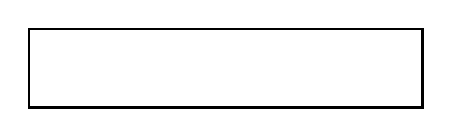
\begin{tikzpicture}
			\draw[black, thick] (0,0) rectangle (5,1);
		\end{tikzpicture}
		\caption{A subfigure}
		\label{fig:sub2}
	\end{subfigure}
	\caption{A figure with two subfigures}
	\label{fig:face_node_centered_discretization_comparison}
\end{figure}